
%(BEGIN_QUESTION)
% Copyright 2007, Tony R. Kuphaldt, released under the Creative Commons Attribution License (v 1.0)
% This means you may do almost anything with this work of mine, so long as you give me proper credit

Regn ut $I$, $U_{C}$, $U_{BC}$ og  $U_{B}$ basert på at transmitteren er kalibrert for et måleområde fra 50mbar til 400mbar. Transmitteren har et utgangssignal på 4-20mA 
Vis alle utregninger. 
$$\includegraphics[width=12cm]{mf001x01.eps}$$


\begin{tikzpicture}
	\draw[step=0.5cm,gray!20,very thin]  grid (16,13) ;
\end{tikzpicture}

%\underbar{file mf001.tex}
%(END_QUESTION)





%(BEGIN_ANSWER)

\begin{itemize}
\item{} $I$ = \underbar{\bf 12} mA
\vskip 10pt
\item{} $U_{C}$ = \underbar{\bf 3} V 
\vskip 10pt
\item{} $U_{BC}$ = \underbar{\bf 17.56} V 
\vskip 10pt
\item{} $U_{B}$ = \underbar{\bf 20.56} V 
\end{itemize}

%(END_ANSWER)





%(BEGIN_NOTES)


%INDEX% Basics, 2-wire loop-powered transmitter: circuit analysis

%(END_NOTES)


